\documentclass{extbook}[14pt]
\usepackage{multicol, enumerate, enumitem, hyperref, color, soul, setspace, parskip, fancyhdr, amssymb, amsthm, amsmath, latexsym, units, mathtools}
\everymath{\displaystyle}
\usepackage[headsep=0.5cm,headheight=0cm, left=1 in,right= 1 in,top= 1 in,bottom= 1 in]{geometry}
\usepackage{dashrule}  % Package to use the command below to create lines between items
\newcommand{\litem}[1]{\item #1

\rule{\textwidth}{0.4pt}}
\pagestyle{fancy}
\lhead{}
\chead{Answer Key for Makeup Progress Quiz 3 Version B}
\rhead{}
\lfoot{1648-1753}
\cfoot{}
\rfoot{Summer C 2021}
\begin{document}
\textbf{This key should allow you to understand why you choose the option you did (beyond just getting a question right or wrong). \href{https://xronos.clas.ufl.edu/mac1105spring2020/courseDescriptionAndMisc/Exams/LearningFromResults}{More instructions on how to use this key can be found here}.}

\textbf{If you have a suggestion to make the keys better, \href{https://forms.gle/CZkbZmPbC9XALEE88}{please fill out the short survey here}.}

\textit{Note: This key is auto-generated and may contain issues and/or errors. The keys are reviewed after each exam to ensure grading is done accurately. If there are issues (like duplicate options), they are noted in the offline gradebook. The keys are a work-in-progress to give students as many resources to improve as possible.}

\rule{\textwidth}{0.4pt}

\begin{enumerate}\litem{
For the graph below, find the value(s) $a$ that makes the statement true: $ \displaystyle \lim_{x \rightarrow a} f(x)$ does not exist.

\begin{center}
    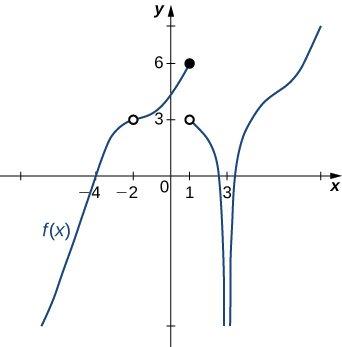
\includegraphics[width=0.5\textwidth]{../Figures/evaluateLimitGraphicallyCopyB.png}
\end{center}


The solution is \( 1 \), which is option B.\begin{enumerate}[label=\Alph*.]
\item \( -2 \)


\item \( 1 \)


\item \( 3 \)


\item \( \text{Multiple } a \text{ make the statement true}. \)


\item \( \text{No } a \text{ make the statement true}. \)


\end{enumerate}

\textbf{General Comment:} \textbf{General Comments:} Remember that the limit does not exist if the left-hand and right-hand limits do not match.
}
\litem{
Evaluate the one-sided limit of the function $f(x)$ below, if possible.
\[ \lim_{x \rightarrow 8^+} \frac{-4}{(x+8)^4}+6 \]The solution is \( f(8) \), which is option B.\begin{enumerate}[label=\Alph*.]
\item \( \infty \)


\item \( f(8) \)


\item \( -\infty \)


\item \( \text{The limit does not exist} \)


\item \( \text{None of the above} \)


\end{enumerate}

\textbf{General Comment:} \textbf{General comments:} You should be able to graph the rational function displayed. If not, go back to Module 7 to learn about the general shape of rational functions.
}
\litem{
Evaluate the limit below, if possible.
\[ \lim_{x \rightarrow 5} \frac{\sqrt{6x - 14} - 4}{7x - 35} \]The solution is \( \text{None of the above} \), which is option E.\begin{enumerate}[label=\Alph*.]
\item \( \infty \)

You likely believed that since the denominator is equal to 0, the limit is infinity.
\item \( 0.350 \)

You likely tried to use a shortcut to find the limit of a function that only works for when the numerator/denominator are polynomials.
\item \( 0.018 \)

You likely learned L'Hospital's Rule in a previous course, but misapplied it here.
\item \( 0.125 \)

You likely memorized how to solve the similar homework problem and used the same formula here.
\item \( \text{None of the above} \)

* This is the correct option as the limit is 0.107.
\end{enumerate}

\textbf{General Comment:} \textbf{General comments:} It is difficult to imagine the graph of this function, so you need to test values close to $x = 5$.
}
\litem{
Evaluate the limit below, if possible.
\[ \lim_{x \rightarrow 6} \frac{\sqrt{6x - 20} - 4}{5x - 30} \]The solution is \( \text{None of the above} \), which is option E.\begin{enumerate}[label=\Alph*.]
\item \( 0.125 \)

You likely memorized how to solve the similar homework problem and used the same formula here.
\item \( 0.025 \)

You likely learned L'Hospital's Rule in a previous course, but misapplied it here.
\item \( 0.490 \)

You likely tried to use a shortcut to find the limit of a function that only works for when the numerator/denominator are polynomials.
\item \( \infty \)

You likely believed that since the denominator is equal to 0, the limit is infinity.
\item \( \text{None of the above} \)

* This is the correct option as the limit is 0.150.
\end{enumerate}

\textbf{General Comment:} \textbf{General comments:} It is difficult to imagine the graph of this function, so you need to test values close to $x = 6$.
}
\litem{
Based on the information below, which of the following statements is always true?

\begin{center}
    \textit{ $f(x)$ approaches $4.192$ as $x$ approaches $1$. }
\end{center}
The solution is \( \text{None of the above are always true.} \), which is option E.\begin{enumerate}[label=\Alph*.]
\item \( f(1) \text{ is close to or exactly } 4 \)


\item \( f(4) \text{ is close to or exactly } 1 \)


\item \( f(4) = 1 \)


\item \( f(1) = 4 \)


\item \( \text{None of the above are always true.} \)


\end{enumerate}

\textbf{General Comment:} The limit tells you what happens as the $x$-values approach $1$. It says \textbf{absolutely nothing} about what is happening exactly at $f(1)$!
}
\litem{
For the graph below, find the value(s) $a$ that makes the statement true: $ \displaystyle \lim_{x \rightarrow a} f(x)$ does not exist.

\begin{center}
    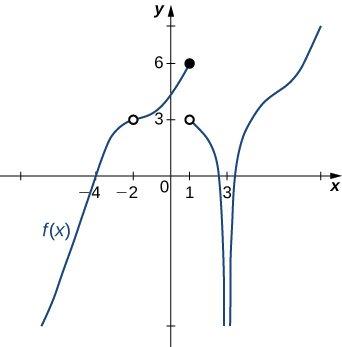
\includegraphics[width=0.5\textwidth]{../Figures/evaluateLimitGraphicallyB.png}
\end{center}


The solution is \( 1 \), which is option B.\begin{enumerate}[label=\Alph*.]
\item \( 3 \)


\item \( 1 \)


\item \( -2 \)


\item \( \text{Multiple } a \text{ make the statement true}. \)


\item \( \text{No } a \text{ make the statement true}. \)


\end{enumerate}

\textbf{General Comment:} \textbf{General Comments:} Remember that the limit does not exist if the left-hand and right-hand limits do not match.
}
\litem{
Evaluate the one-sided limit of the function $f(x)$ below, if possible.
\[ \lim_{x \rightarrow -1^+} \frac{6}{(x+1)^4}+7 \]The solution is \( \infty \), which is option C.\begin{enumerate}[label=\Alph*.]
\item \( f(-1) \)


\item \( -\infty \)


\item \( \infty \)


\item \( \text{The limit does not exist} \)


\item \( \text{None of the above} \)


\end{enumerate}

\textbf{General Comment:} \textbf{General comments:} You should be able to graph the rational function displayed. If not, go back to Module 7 to learn about the general shape of rational functions.
}
\litem{
Based on the information below, which of the following statements is always true?

\begin{center}
    \textit{ As $x$ approaches $0$, $f(x)$ approaches $15.316$. }
\end{center}
The solution is \( f(x) \text{ is close to or exactly } 15.316 \text{ when } x \text{ is close to } 0 \), which is option C.\begin{enumerate}[label=\Alph*.]
\item \( f(x) \text{ is close to or exactly } 0 \text{ when } x \text{ is close to } 15.316 \)


\item \( f(x) = 0 \text{ when } x \text{ is close to } 15.316 \)


\item \( f(x) \text{ is close to or exactly } 15.316 \text{ when } x \text{ is close to } 0 \)


\item \( f(x) = 15.316 \text{ when } x \text{ is close to } 0 \)


\item \( \text{None of the above are always true.} \)


\end{enumerate}

\textbf{General Comment:} The limit tells you what happens as the $x$-values approach $0$. It says \textbf{absolutely nothing} about what is happening exactly at $f(0)$!
}
\litem{
To estimate the one-sided limit of the function below as $x$ approaches 5 from the right, which of the following sets of numbers should you use?
\[ \frac{\frac{5}{x} - 1}{x - 5} \]The solution is \( \{ 5.1000, 5.0100, 5.0010, 5.0001 \} \), which is option E.\begin{enumerate}[label=\Alph*.]
\item \( \{ 4.9000, 4.9900, 4.9990, 4.9999 \} \)

These values would estimate the limit of 5 on the left.
\item \( \{ 5.0000, 5.1000, 5.0100, 5.0010 \} \)

If we get $\frac{0}{0}$ or $\frac{\infty}{\infty}$, the value 5 doesn't help us estimate the limit.
\item \( \{ 5.0000, 4.9000, 4.9900, 4.9990 \} \)

If we get $\frac{0}{0}$ or $\frac{\infty}{\infty}$, the value 5 doesn't help us estimate the limit.
\item \( \{ 4.9000, 4.9900, 5.0100, 5.1000 \} \)

These values would estimate the limit at the point and not a one-sided limit.
\item \( \{ 5.1000, 5.0100, 5.0010, 5.0001 \} \)

This is correct!
\end{enumerate}

\textbf{General Comment:} \textbf{General Comments:} To evaluate a one-sided limit, we want to put numbers close to the limit. We can't use the limit value itself if it results in $\frac{0}{0}$ or $\frac{\infty}{\infty}$
}
\litem{
To estimate the one-sided limit of the function below as $x$ approaches 6 from the left, which of the following sets of numbers should you use?
\[ \frac{\frac{6}{x} - 1}{x - 6} \]The solution is \( \{ 5.9000, 5.9900, 5.9990, 5.9999 \} \), which is option E.\begin{enumerate}[label=\Alph*.]
\item \( \{ 5.9000, 5.9900, 6.0100, 6.1000 \} \)

These values would estimate the limit at the point and not a one-sided limit.
\item \( \{ 6.1000, 6.0100, 6.0010, 6.0001 \} \)

These values would estimate the limit of 6 on the right.
\item \( \{ 6.0000, 6.1000, 6.0100, 6.0010 \} \)

If we get $\frac{0}{0}$ or $\frac{\infty}{\infty}$, the value 6 doesn't help us estimate the limit.
\item \( \{ 6.0000, 5.9000, 5.9900, 5.9990 \} \)

If we get $\frac{0}{0}$ or $\frac{\infty}{\infty}$, the value 6 doesn't help us estimate the limit.
\item \( \{ 5.9000, 5.9900, 5.9990, 5.9999 \} \)

This is correct!
\end{enumerate}

\textbf{General Comment:} \textbf{General Comments:} To evaluate a one-sided limit, we want to put numbers close to the limit. We can't use the limit value itself if it results in $\frac{0}{0}$ or $\frac{\infty}{\infty}$
}
\end{enumerate}

\end{document}